\documentclass[tikz,border=4pt]{standalone}
\begin{document}
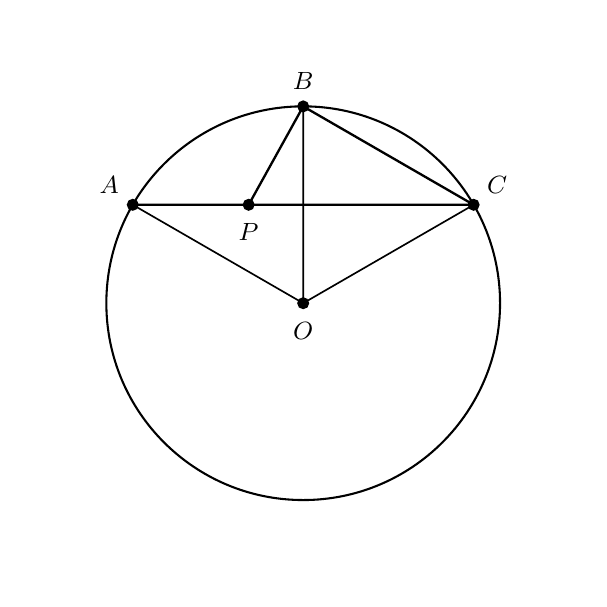
\begin{tikzpicture}[x=0.025cm,y=-0.025cm]
\path[use as bounding box] (0,0) rectangle (280,280);
\path[draw=black,fill=none,line width=.75pt] (140,140) circle[radius=2.5cm];
\path[draw=black,fill=none,line width=0.6pt,line join=round] (53.3975,90) -- (140,140) -- (140,40);
\path[draw=black,fill=none,line width=0.6pt,line join=round] (140,140) -- (226.6025,90);
\path[draw=black,fill=none,line width=0.84pt,line join=round] (53.3975,90) -- (226.6025,90) -- (140,40) -- (112.2872,90);
\path[draw=black,fill=black,line width=.75pt] (53.3975,90) circle[radius=0.0625cm];
\node[font=\small,inner sep=0pt] at (41.3975,80) {$A$};
\path[draw=black,fill=black,line width=.75pt] (140,40) circle[radius=0.0625cm];
\node[font=\small,inner sep=0pt] at (140,27) {$B$};
\path[draw=black,fill=black,line width=.75pt] (226.6025,90) circle[radius=0.0625cm];
\node[font=\small,inner sep=0pt] at (238.6025,80) {$C$};
\path[draw=black,fill=black,line width=.75pt] (112.2872,90) circle[radius=0.0625cm];
\node[font=\small,inner sep=0pt] at (112.2872,104) {$P$};
\path[draw=black,fill=black,line width=.75pt] (140,140) circle[radius=0.0625cm];
\node[font=\small,inner sep=0pt] at (140,154) {$O$};
\end{tikzpicture}
\end{document}
